
%--------------------------------------------------------------------------------
% Constrói a capa com base na seção de identificação do main.tex
%--------------------------------------------------------------------------------
\begin{capa}
    \setlength{\belowcaptionskip}{0pt}
    \setlength{\abovecaptionskip}{0pt}
    \setlength{\intextsep}{-18pt}
        \begin{figure}[h]
    		\begin{center}
    		    
\includegraphics[scale=.5]{img/NEW_LOGO_UNIVASF.jpg}
    		\end{center}
    	\end{figure}

        %
\includegraphics[scale=0.6]{img/univasf.jpg}
        \center
    	{\ABNTEXchapterfont\large\imprimirinstituicao}

    	\vspace*{2cm}
    	    {\imprimirautor}
    	\vspace*{2cm}
        \begin{center}
    		\ABNTEXchapterfont\bfseries\large\imprimirtitulo
        \end{center}
    	\vfill

    	\ABNTEXchapterfont\bfseries\large\imprimirlocal\\
    	\the\year

    	\vspace*{1cm}
\end{capa}
%--------------------------------------------------------------------------------
% Constrói a folha de rosto com base na seção de identificação do main.tex
%--------------------------------------------------------------------------------
\begin{folhaderosto}
    \center
    	{\ABNTEXchapterfont\large\imprimirinstituicao}

		\vspace*{2cm}
    	    {\imprimirautor}
    	\vspace*{2cm}
		\vspace*{\fill}

		{\ABNTEXchapterfont\bfseries\large\imprimirtitulo}
		\vspace*{\fill}

		{\hspace{.45\textwidth}
		\begin{minipage}{.5\textwidth}
			\SingleSpacing
			\imprimirpreambulo \\ \\

			{\imprimirorientadorRotulo~\imprimirorientador\par}
			{\imprimircoorientadorRotulo~\imprimircoorientador\par}

		\end{minipage}%
		\vspace*{\fill}}%
		\vspace*{\fill}
			\ABNTEXchapterfont\bfseries\large\imprimirlocal\\
			\the\year
		\vspace*{1cm}
\end{folhaderosto}

%--------------------------------------------------------------------------------
% Constrói a ficha catalográfia com base na seção de identificação do main.tex
% Está comentado porque no final das contas a biblioteca do seu campus que gera a
% numeração, você pode adicionar os numeros aqui, ou anexar o pdf gerado por eles
% ao documento.
%--------------------------------------------------------------------------------
%\begin{fichacatalografica}
%	\vspace*{\fill}					% Posição vertical
%	\hrule							% Linha horizontal
%	\begin{center}					% Minipage Centralizado
%	\begin{minipage}[c]{12.5cm}		% Largura
%
%	\imprimirautor
%
%	\hspace{0.5cm} \imprimirtitulo  / \imprimirautor. --
%	\imprimirlocal, \the\year-
%
%	\hspace{0.5cm} xx p. : il. (algumas color.) ; 30 cm.\\
%
%	\hspace{0.5cm} \imprimirorientadorRotulo~\imprimirorientador\\
%
%	\hspace{0.5cm}
%	\parbox[t]{\textwidth}{\imprimirtipotrabalho~--~\imprimirinstituicao,
%	\the\year.}\\
%
%	\hspace{0.5cm}
%		1. Palavra-chave1.
%		2. Palavra-chave2.
%		I. Orientador.
%		II. Universidade xxx.
%		III. Faculdade de xxx.
%		IV. Título\\
%
%	\hspace{8.75cm} CDU 02:141:005.7\\
%
%	\end{minipage}
%	\end{center}
%	\hrule
%\end{fichacatalografica}

%--------------------------------------------------------------------------------
% Anexando a ficha catalogáfica e a folha de aprovação
%--------------------------------------------------------------------------------

\includepdf[pages=-]{anexos/ficha.pdf}

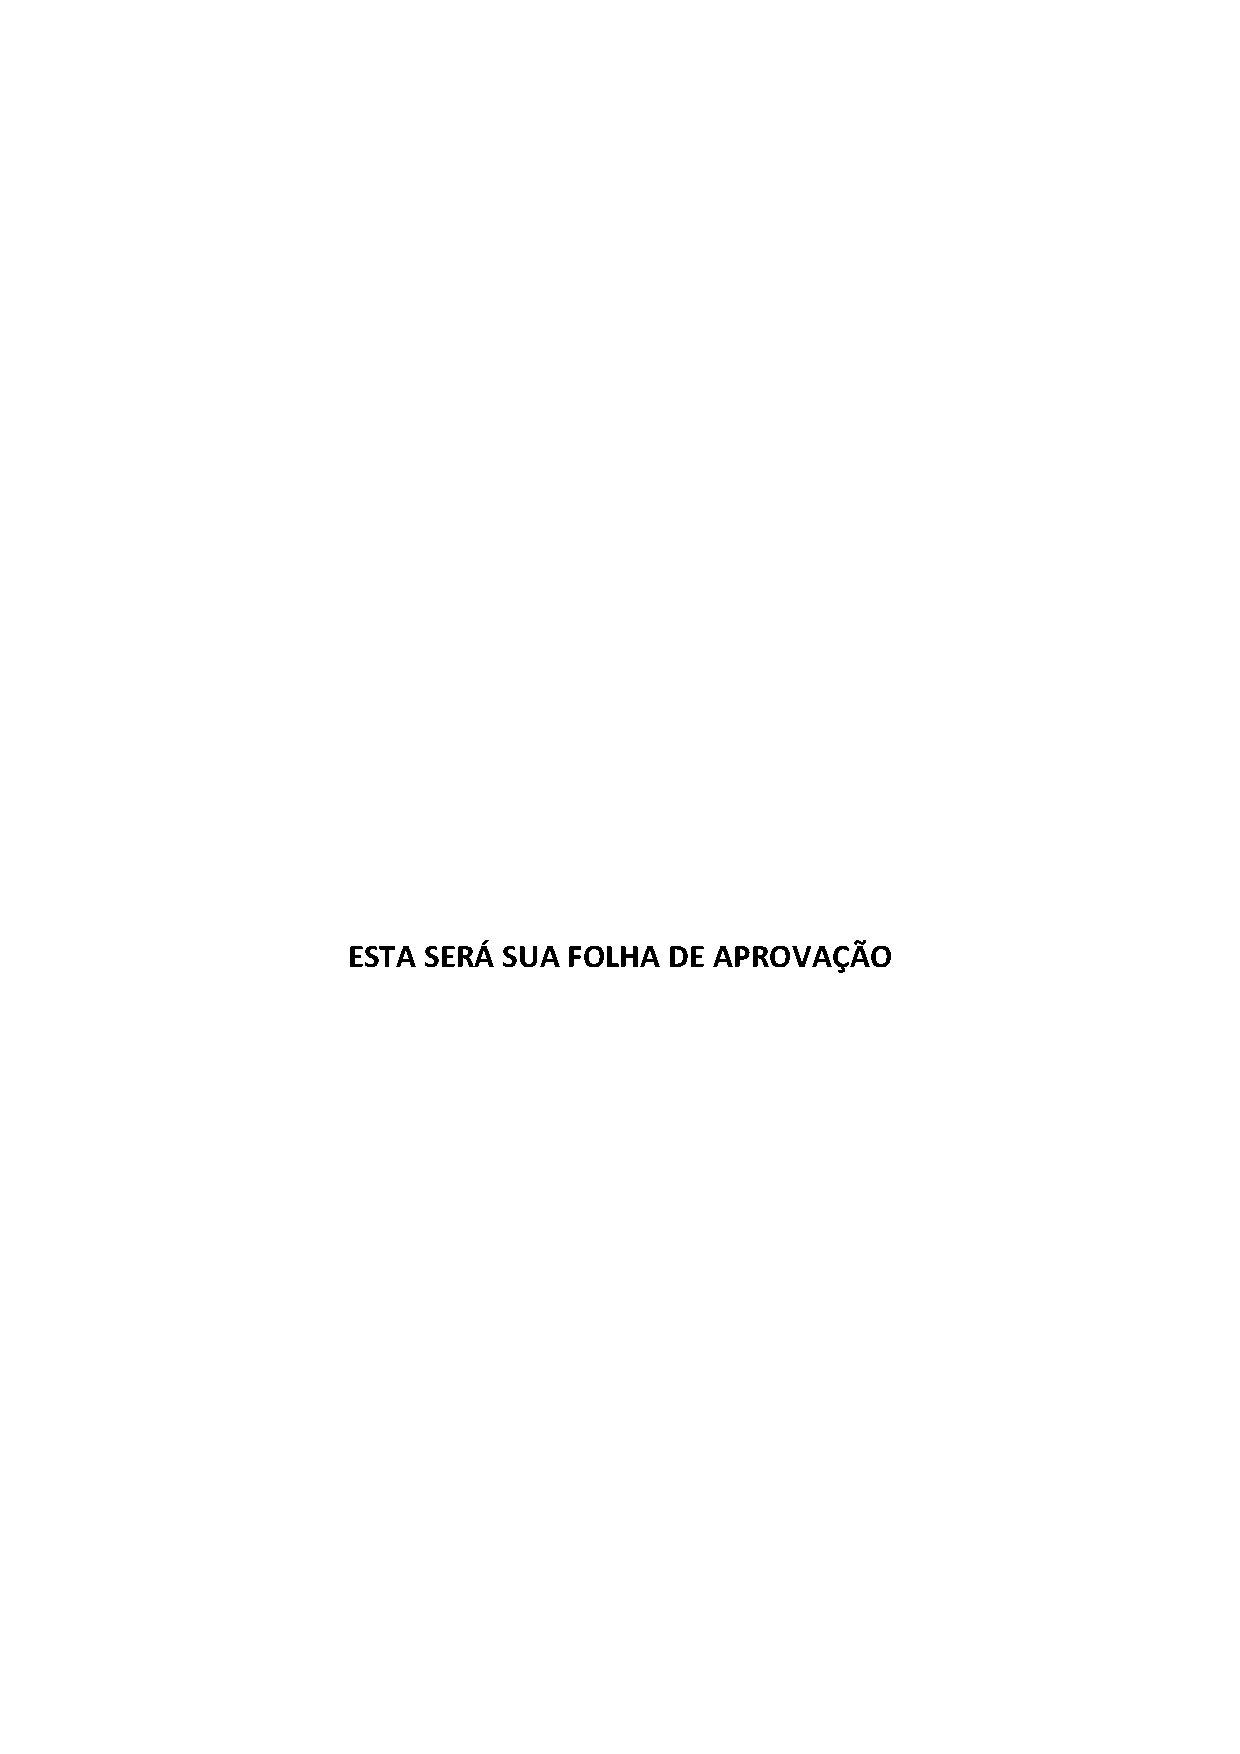
\includepdf[pages=-]{anexos/aprovacao.pdf}

%%--------------------------------------------------------------------------------
% Insere a folha de aprovação 
%--------------------------------------------------------------------------------
\begin{folhadeaprovacao}
	\begin{center}
		{\ABNTEXchapterfont\bfseries\large\imprimirinstituicao}
		\vspace*{\fill}

		{\ABNTEXchapterfont\bfseries\large FOLHA DE APROVAÇÃO}
		\vspace*{\fill}

		{\ABNTEXchapterfont\bfseries\large\imprimirautor}

		\vspace*{\fill}\vspace*{\fill}
		{\ABNTEXchapterfont\bfseries\large\imprimirtitulo}
		\vspace*{\fill}

		{\hspace{.45\textwidth}
		\begin{minipage}{.5\textwidth}
			\SingleSpacing
			\ABNTEXchapterfont\imprimirpreambulo \\ \\

			% {\ABNTEXchapterfont\imprimirorientadorRotulo~\imprimirorientador\par}
			% {\ABNTEXchapterfont\imprimircoorientadorRotulo~\imprimircoorientador\par}

		\end{minipage}%
		\vspace*{\fill}}
	\end{center}

	\vspace*{\fill}	
	
	\begin{center}
		% \ABNTEXchapterfont\large Aprovado em: \_\_\_\_ de \_\_\_\_\_\_\_\_ de 2020.
		\ABNTEXchapterfont\large Aprovado em: de de 2022.
	\end{center}

	\vspace*{\fill}
	
	\begin{center}
			 \ABNTEXchapterfont\bfseries\large Banca Examinadora
	\end{center}
		
	\ABNTEXchapterfont\assinatura{Rosalvo Ferreira de Oliveira Neto, Doutor, Universidade Federal do Vale do São Francisco}	
	\ABNTEXchapterfont\assinatura{Juracy Emanuel Magalhães da Franca, Mestre, Universidade Federal do Vale do São Francisco}
	\ABNTEXchapterfont\assinatura{Marcus Vinícius Midena Ramos, Doutor, Universidade Federal do Vale do São Francisco}
	\vspace*{\fill}

	 
\end{folhadeaprovacao}

\setlength{\ABNTEXsignwidth}{12cm}

%--------------------------------------------------------------------------------
% Está comentado pelo mesmo motivo da ficha catalográfica
%--------------------------------------------------------------------------------
%\begin{folhadeaprovacao}
%	\begin{center}
%	    {\ABNTEXchapterfont\bfseries\large\imprimirinstituicao}
%	    \vspace*{\fill}
%
%	    {\ABNTEXchapterfont\bfseries\large FOLHA DE APROVAÇÃO}
%	    \vspace*{\fill}
%
%	    {\ABNTEXchapterfont\bfseries\large\imprimirautor}
%
%	    \vspace*{\fill}\vspace*{\fill}
%	    {\ABNTEXchapterfont\bfseries\large\imprimirtitulo}
%	    \vspace*{\fill}
%
%	    {\hspace{.45\textwidth}
%		\begin{minipage}{.5\textwidth}
%			\SingleSpacing
%			\ABNTEXchapterfont\imprimirpreambulo \\ \\
%
%			{\ABNTEXchapterfont\imprimirorientadorRotulo~\imprimirorientador\par}
%			{\ABNTEXchapterfont\imprimircoorientadorRotulo~\imprimircoorientador\par}
%
%		\end{minipage}%
%	    \vspace*{\fill}}
%	\end{center}
%
%	\vspace*{\fill}
%
%	\begin{center}
%			 \ABNTEXchapterfont\large Aprovado em: \_\_\_\_ de \_\_\_\_ de 2017
%	\end{center}

%	\vspace*{\fill}

%	\begin{center}
%			 \ABNTEXchapterfont\bfseries\large Banca Examinadora
%	\end{center}
%
%   \ABNTEXchapterfont\assinatura{Fábio Nelson de Sousa Pereira, Mestre, Universidade Federal do Vale do São Francisco}
%	\ABNTEXchapterfont\assinatura{Jorge Luis Cavalcanti Ramos, Doutor, Universidade Federal do vale do São Francisco}
%  \ABNTEXchapterfont\assinatura{Ricardo Argenton Ramos, Doutor, Universidade Federal do Vale do São Francisco}
%	 \vspace*{\fill}


%\end{folhadeaprovacao}

%--------------------------------------------------------------------------------
% Insere a epígrafe
%--------------------------------------------------------------------------------
\newpage
\vspace*{\fill}
\begin{flushright}
		
\end{flushright}

%--------------------------------------------------------------------------------
% Seção de agradecimentos
%--------------------------------------------------------------------------------
\begin{agradecimentos}
Eu agradeço primeiramente a Deus, por ter me permitido chegar até aqui com alegria e saúde. Aos meus pais Edeilton e Iolanda que me apoiaram durante tanto tempo. Agradeço  aos meus colegas da universidade, no qual tive várias conversas interessantes ao longo da minha graduação. Agradeço aos professores das mais diversas disciplinas, tanto do colegiado de Engenharia da computação como também do colegiado de engenharia elétrica, pelo conhecimento compartilhado e ajuda oferecida, que me fez abrir os olhos e aumentar ainda mais a minha curiosidade sobre as diversas áreas do  conhecimento. Agradeço ao meu orientador Max Santana, que aceitou me ajudar nesse trabalho de conclusão de curso, a Ruan de Medeiros e Ricado Argenton, por aceitarem ser avaliadores da banca de defesa. 
%lipsum[2-4]

\end{agradecimentos}

%--------------------------------------------------------------------------------
% Insere a segunda epígrafe
%--------------------------------------------------------------------------------
\begin{epigrafe}
    \vspace*{\fill}
	\begin{flushright}
		Se pude enxergar a tão grande distância, foi subindo nos ombros de gigantes.\\
		 \vspace{\baselineskip}
		\textbf{Isaac Newton}\\
		\textbf{Carta à Robert Hooke, 1676}
	\end{flushright}
\end{epigrafe}



%--------------------------------------------------------------------------------
% Seção de resumos
%--------------------------------------------------------------------------------
% resumo em português
\setlength{\absparsep}{18pt} % ajusta o espaçamento dos parágrafos do resumo
\begin{resumo}


Uma das fases mais importantes no desenvolvimento de minifoguetes depois da simulação é o teste prático. Esta fase validará de fato o desempenho que foi simulado, mas para isso é necessário ter um sistema embarcado dentro do minifoguete capaz de capturar as principais variáveis, armazená-las e transmiti-las para um computador em solo. A fim de contribuir com a equipe de foguetemodelismo chamada Cactus Rocket Design da Universidade Federal do Vale do São Francisco, este trabalho tem como objetivo a construção de dois sistemas. O primeiro sistema embarcado será responsável pela captura, armazenamento e envio por telemetria dos principais dados sobre o minifoguete. Já o segundo sistema será responsável por receber os dados e transmitir para um computador, para que possa ser armazenado em um arquivo txt, para futuros relatórios. Assim, evita-se a perda dos dados gravados no cartão micro SD caso ocorra à perda do foguete.









 \textbf{Palavras-chave}: \textit{Minifoguete, Sistema Embarcado, Cactus Rocket Design, Telemetria}.

\end{resumo}

%---------------------------------------------------------------------------------
% resumo em inglês
\begin{resumo}[Abstract]
\begin{otherlanguage*}{english}



One of the most important phases in the development of mini-rockets after the simulation is the practical test. This phase will in fact validate the performance that was simulated, but for that it is necessary to have an embedded system inside the mini-rocket capable of capturing the main variables, storing them and transmitting them to a computer on the ground. In order to contribute to the model rocket team called Cactus Rocket Design at the Universidade Federal do Vale do São Francisco, this work aims to build two systems. The first embedded system will be responsible for capturing, storing and telemetry sending the main data about the mini-rocket. The second system will be responsible for receiving the data and transmitting it to a computer, so that it can be stored in a txt file for future reports. Thus, the loss of data recorded on the micro SD card is avoided if the rocket is lost. 







	\vspace{\onelineskip}

	\noindent
	\textbf{Key-words}: \textit{mini-rocket, Embedded System, Cactus Rocket Design, Telemetry  }.

\end{otherlanguage*}
\end{resumo}


%---------------------------------------------------------------------------------
% Insere lista de ilustrações
%---------------------------------------------------------------------------------
\begin{KeepFromToc} % Este comando evita que todas as seções dentro dele de apareçam no sumário
\pdfbookmark[0]{\listfigurename}{lof}
\listoffigures
%\addcontentsline{toc}{chapter}{Lista de Figuras}
\cleardoublepage


%---------------------------------------------------------------------------------
% Insere lista de tabelas
%---------------------------------------------------------------------------------
\pdfbookmark[0]{\listtablename}{lot}
\listoftables
\cleardoublepage

%---------------------------------------------------------------------------------
% Insere lista de quadros
%---------------------------------------------------------------------------------
%\pdfbookmark[0]{\listofquadrosname}{loq}
%\listofquadros*
%\cleardoublepage

%---------------------------------------------------------------------------------
% Ajusta lista de código - alterar de figures para códigos - by @Gabrielr2508
%---------------------------------------------------------------------------------
\makeatletter
\let\l@listing\l@figure
\def\newfloat@listoflisting@hook{\let\figurename\listingname}
\makeatother

%---------------------------------------------------------------------------------
% Insere lista de códigos - by @leolleocomp
%---------------------------------------------------------------------------------
%\listoflistings

\end{KeepFromToc}

%---------------------------------------------------------------------------------
% Insere lista de abreviaturas e siglas
%---------------------------------------------------------------------------------







\begin{siglas}




%###    a    ###
%###    b    ###
\item[BAR] Brazilian Association of Rocketry (Associação Brasileira de Minifoguetes)
%###    c    ###
\item[CI] Circuito Integrado
\item[CTA] Centro Técnico Aeroespacial 
%###    d    ###
\item[DCTA] Departamento de Ciência e Tecnologia Aeroespacial 
\item[DOP] Dilution of precision (Diluição da precisão, ou diluição geométrica da precisão)
%###    e    ###
%###    f    ###
\item[FM] Foguetemodelo 
%###    g    ###
\item[GPS] Sistema de Posicionamento Global 
%###    h    ###
%###    i    ###
\item[ITA]  Instituto Tecnológico de Aeronáutica
%###    j    ###
%###    k    ###
%###    l    ###
%###    m    ###
\item[MFE] Minifoguete experimental 
%###    n    ###
%###    o    ###
%###    p    ###
\item[PCB] Printed Circuit Board (Placa de Circuito Impresso)
%###    q    ###
%###    r    ###
%###    s    ###
\item[SNR] Signal to Noise Ratio (Razão sinal ruído) 
%###    t    ###
%###    u    ###
%###    v    ###
\item[VLM-1] Veículo lançador de microssatélites
\item[VPP] Peak-to-peak voltage (tensão de pico a pico)
\item[VLS] Veículo lançador de satélites
%###    w    ###
%###    x    ###
%###    y    ###
%###    z    ###



\end{siglas}




%\begin{siglas}
%	\item[LI]       Lorem Ipsum
%    \item[LII]		Lorem Ipsum Ipsum

%\end{siglas}

%---------------------------------------------------------------------------------
% Insere o sumario
%---------------------------------------------------------------------------------
\pdfbookmark[0]{\contentsname}{toc}
\tableofcontents*
\cleardoublepage


